\documentclass [12pt]{article}


\usepackage{ucs}
\usepackage[utf8x]{inputenc} %Поддержка UTF8
\usepackage{cmap} % Улучшенный поиск русских слов в полученном pdf-файле
\usepackage[english,russian]{babel} %Пакет для поддержки русского и английского языка
\usepackage{graphicx} %Поддержка графиков
\usepackage{float} %Поддержка float-графиков
\usepackage[left=20mm,right=15mm, top=20mm,bottom=20mm,bindingoffset=0cm]{geometry}
\usepackage{mathtools} 
\usepackage{amsmath}
\usepackage{setspace,amsmath}
\usepackage{amsmath,amssymb}
\usepackage{dsfont}
\renewcommand{\baselinestretch}{1.2}
 
\usepackage{color} 
\definecolor{deepblue}{rgb}{0,0,0.5}
\definecolor{deepred}{rgb}{0.6,0,0}
\definecolor{deepgreen}{rgb}{0,0.5,0}

\DeclareFixedFont{\ttb}{T1}{txtt}{bx}{n}{12} % for bold
\DeclareFixedFont{\ttm}{T1}{txtt}{m}{n}{12}  % for normal

\usepackage{listings}
 
\lstset{
	language=Python,
	basicstyle=\ttm,
	otherkeywords={self},             % Add keywords here
	keywordstyle=\ttb\color{deepblue},
	emph={MyClass,__init__},          % Custom highlighting
	emphstyle=\ttb\color{deepred},    % Custom highlighting style
	stringstyle=\color{deepgreen},
	frame=tb,                         % Any extra options here
	showstringspaces=false            % 
}
 
\usepackage{hyperref}
 
\hypersetup{
    bookmarks=true,         % show bookmarks bar?
    unicode=false,          % non-Latin characters in Acrobat’s bookmarks
    pdftoolbar=true,        % show Acrobat’s toolbar?
    pdfmenubar=true,        % show Acrobat’s menu?
    pdffitwindow=false,     % window fit to page when opened
    pdfstartview={FitH},    % fits the width of the page to the window
    pdftitle={My title},    % title
    pdfauthor={Author},     % author
    pdfsubject={Subject},   % subject of the document
    pdfcreator={Creator},   % creator of the document
    pdfproducer={Producer}, % producer of the document
    pdfkeywords={keyword1} {key2} {key3}, % list of keywords
    pdfnewwindow=true,      % links in new PDF window
    colorlinks=true,       % false: boxed links; true: colored links
    linkcolor=black,          % color of internal links (change box color with linkbordercolor)
    citecolor=green,        % color of links to bibliography
    filecolor=magenta,      % color of file links
    urlcolor=cyan           % color of external links
}

\title{}
\date{}
\author{}

\begin{document}
\begin{titlepage}
\thispagestyle{empty}
\begin{center}
Федеральное государственное бюджетное образовательное учреждение высшего профессионального образования \\Московский государственный технический университет имени Н.Э. Баумана

\end{center}
\vfill
\centerline{\large{Лабораторная работа №5}}
\centerline{\large{по курсу <<Численные методы>>}}
\centerline{\large{<<Метод наименьших квадратов. Аппроксимация алгебраическими многочленами>>}}
\vfill
\hfill\parbox{5cm} {
           Выполнил:\\
           студент группы ИУ9-62Б \hfill \\
           Головкин Дмитрий\hfill \medskip\\
           Проверила:\\
           Домрачева А.Б.\hfill
       }
\centerline{Москва, 2023}
\clearpage
\end{titlepage}

\textsc{\textbf{Цель:}} 

Анализ метода метода наименьших квадратов для решения задачи аппроксимации.

\textsc{\textbf{Постановка задачи:}} 

\textbf{Дано:}  Функция $y_i = f(x_i),  i = \overline{0,n}$ задана таблично, исходные данные включают ошибки измерения.

\begin{table}[h]
\begin{center}
\begin{tabular}{|c|c|c|c|c|}
\hline
$x_1$ & $x_2$ & ... & $x_{n-1}$ & $x_n$ \\
\hline
$y_1$ & $y_2$ & ... & $y_{n-1}$ & $y_n$ \\
\hline
\end{tabular}
\end{center}
\end{table}

\textbf{Найти:} Гладкую аналитическую функцию  $z(x)$, доставляющую наименьшее значение величине $$ MSE=\sqrt[2]{\sum\limits_{i = 0}^n{(z(x_i) - y_i)^2}}$$ Эту величину называют среднеквадратичным уклонением функции $z(x)$ от системы узлов. Описанный подход к решению задачи приближения функции - методом наименьших квадратов.

\textbf{Тестовый пример:} 

Зададим некоторую функцию $f(x) = y$. Представим значения в виде таблицы:

\begin{table}[h]
\begin{center}
\begin{tabular}{|c|c|c|c|c|c|c|c|c|c|}
\hline
1 & 1.5 & 2 & 2.5 & 3 & 3.5 & 4 & 4.5 & 5\\
\hline
0.16 & 0.68 & 1.96 & 2.79 & 3.80 & 6.81 & 9.50 & 15.60 & 24.86\\
\hline
\end{tabular}
\end{center}
\end{table}

\textbf{Описание метода:}

Как правило, $z(x)$ отыскивают в виде линейной комбинации заданных функций $$ z(x) = \lambda_{1}\phi_{1}(x) + ... + \lambda_m\phi_m(x) $$
Параметры $\lambda_i, i = \overline{1,m}$ являются решениями линейной системы наименьших квадратов $$ A\lambda = b $$,
где $\lambda$ - столбец параметров $\lambda_i$ . $A = (a_ij)$ - симметричная положительно определенная матрица (матрица Грама) с коэффициентами $ a_ij = \sum\limits_{k = 0}^n{\phi_i(x_i)\phi_j(x_k)}$; b - столбец правой части системы, $ b_i = \sum\limits_{k = 0}^n{\phi_i(x_k)y_k}, \quad i,j = \overline{1,m} $


Если приближаемая функция достаточно глабкая, хотя вид ее и неизвестен, аппроксимирующую функцию нередко ищут в виде алгебраического многочлена $$ z(x) = \lambda_{1} + \lambda_{2}x + ... + \lambda_{m}x^(m-1) $$.
Тогда $\phi_i = x^(i-1)$ и элементы матрица Грама получают по формулам $$ a_ij = \sum\limits_{k = 0}^n{x_{k}^(i + j - 2)}$$,
а свободные члены - $$b_i = \sum\limits_{k = 0}^n{y_{k}^(i - 1)}, \quad i, j = \overline{1,m} $$

Абсолютной погрешностью аппроксимации служит среднеквадратичное отклонение (СКО): $$ \Delta = \frac{MSE}{\sqrt[2]{n}} = \frac{1}{\sqrt[2]{n}}\sqrt[2]{\sum\limits_{k = 0}^n{(y_k - \lambda_{1} - \lambda_{2}x_k - ... -\lambda_{m}x_{k}^(m-1))^2}} $$, 
относительная ошибка $$ \delta = \frac{\Delta}{||y||} = \frac{\Delta}{\sqrt[2]{\sum\limits_{k = 0}^n{y_{k}^2}}} $$

\textsc{\textbf{Практическая реализация:}}
Листинг 1. Аппроксимация функции алгебраическими многочленами
\begin{lstlisting}[language=python]
#!python
# -*- coding: utf-8 -*-
import numpy as np

def func(x):
    return x**2 + np.exp(x)

x = np.array([1,1.5,2,2.5,3,3.5,4,4.5,5])
y = np.array([0.16, 0.68, 1.96, 2.79, 3.80, 6.81, 9.50, 15.60, 24.86])
y = func(x)
n = len(x)
m = 4

a = np.array([[sum(x**(i + j - 2)) for j in range(1,m+1)] for i in range(1,m+1)])
a

b = np.array([sum(y*x**(i - 1)) for i in range(1,m+1)])
b

lambd = np.dot(np.linalg.inv(a), b)
lambd

x_help = np.array([x**i for i in range(m)])
x_help = np.array([sum(-lambd*[x[j]**i for i in range(m)]) for j in range(n)])
x_help

delta = 1 / np.sqrt(n) * np.sqrt(sum((y + x_help)**2))
delta

sigma = delta / np.sqrt(np.sum(y**2))
sigma

x_inner = (x[:-1] + x[1:]) / 2
z = [sum(lambd*[x_in**i for i in range(m)]) for x_in in x_inner]
z

import matplotlib.pyplot as plt
fig, ax = plt.subplots(figsize= (10,8))
ax.plot(x, y, label='true')
ax.plot(x_inner, z, label='aprox')
ax.legend()

\end{lstlisting}
\textbf{Результаты:}

Программа проверялась на тестовом примере, а также в случае, когда функция была задана следующим образом $ f(x) = x^2 + e{^x}$

В результате работы программы (Листинг 1) на тестовом примере получаем следующие результаты: 

\[
  a_{4\times 4} = 
  \begin{pmatrix}
    9.00000000e+00 & 2.70000000e+01 & 9.60000000e+01 & 3.78000000e+02\\
    2.70000000e+01 & 9.60000000e+01 & 3.78000000e+02 & 1.58325000e+03\\
    9.60000000e+01 & 3.78000000e+02 & 1.58325000e+03 & 6.90075000e+03\\
    3.78000000e+02 & 1.58325000e+03 & 6.90075000e+03 & 3.09125625e+04
  \end{pmatrix}
\]
\[
  b_{1\times 4} = 
  \begin{pmatrix}
    66.16 \\
    279.81 \\
    1233.99 \\
    5593.3575 
  \end{pmatrix}
\]
\[
  \lambda_{1\times 4} = 
  \begin{pmatrix}
    -6.65857143 \\
    10.21479076 \\
    -4.4008658 \\
    0.72161616 
  \end{pmatrix}
\]

Значение среднеквадратичного отклонения $\Delta = 0.3737351604786069$ и тогда относительная ошибка $\delta = 0.011676034955305238$

Также была проведена аппроксимация функции в точках, лежаших между опорными. Получаем следующие значения:

\begin{center}
\begin{tabular}{|c|c|}
    \hline
    $x_n$ & $z(x_n)$ \\ \hline
    1.25 & 0.6429707792210024 \\ \hline
    1.75 & 1.6070725108233432 \\ \hline
    2.25 & 2.2649837662344794 \\ \hline
    2.75 & 3.1579166666664946 \\ \hline
    3.25 & 4.827083333331473 \\ \hline
    3.75 & 7.813695887441497 \\ \hline
    4.25 & 12.658966450208652 \\ \hline
    4.75 & 19.90410714284502 \\ \hline
\end{tabular}
\end{center}

\begin{figure}[H]
    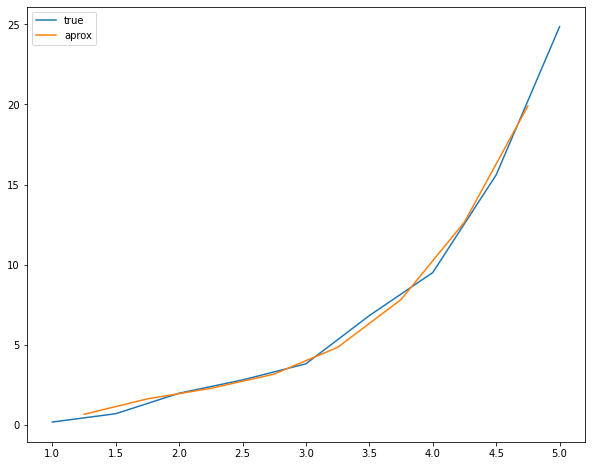
\includegraphics[width=\linewidth]{test_func.png}
    \caption{Графики истинной и приближенной тестовой функции}
    \label{fig:graph1}
\end{figure}

В результате работы программы (Листинг 1) примере с использованием функции из прошлой лабораторной работы получаем следующие результаты: 

\[
  a_{4\times 4} = 
  \begin{pmatrix}
    9.00000000e+00 & 2.70000000e+01 & 9.60000000e+01 & 3.78000000e+02\\
    2.70000000e+01 & 9.60000000e+01 & 3.78000000e+02 & 1.58325000e+03\\
    9.60000000e+01 & 3.78000000e+02 & 1.58325000e+03 & 6.90075000e+03\\
    3.78000000e+02 & 1.58325000e+03 & 6.90075000e+03 & 3.09125625e+04
  \end{pmatrix}
\]
\[
  b_{1\times 4} = 
  \begin{pmatrix}
    469.00095028 \\
    1974.37134166 \\
    8694.92929962 \\
    39378.92997873 
  \end{pmatrix}
\]
\[
  \lambda_{1\times 4} = 
  \begin{pmatrix}
    -29.71590847 \\
    51.51145182 \\
    -23.75591421 \\
    4.30212352 
  \end{pmatrix}
\]

Значение среднеквадратичного отклонения $\Delta = 1.656394535831396$ и тогда относительная ошибка $\delta = 0.007360106164402812$

Также была проведена аппроксимация функции в точках, лежаших между опорными. Получаем следующие значения:

\begin{center}
\begin{tabular}{|c|c|}
    \hline
    $x_n$ & $z(x_n)$ \\ \hline
    1.25 & 5.95737536419831 \\ \hline
    1.75 & 10.733338207589302 \\ \hline
    2.25 & 14.924418191884996 \\ \hline
    2.75 & 21.757207959002912 \\ \hline
    3.25 & 34.458300150860595 \\ \hline
    3.75 & 56.25428740937559 \\ \hline
    4.25 & 90.37176237646543 \\ \hline
    4.75 & 140.0373176940476 \\ \hline
\end{tabular}
\end{center}

\begin{figure}[H]
    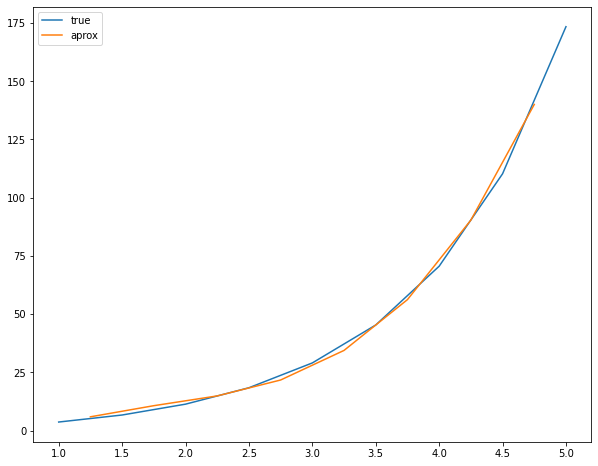
\includegraphics[width=\linewidth]{test_func2.png}
    \caption{Графики истинной и приближенной тестовой функции}
    \label{fig:graph2}
\end{figure}

\textbf{Выводы:}

В ходе выполнения лабораторной работы был рассмотрен метод аппроксимации алгебраическими многочленами и метод наименьших квадратов. Для этих методов была написана реализация на языке программирования Python. Анализируя результаты полученной программы, можно заметить, что данные методы уже для кубических многочленов дают достаточно неплохую аппроксимацию исходной функции. Дальнейшее увеличение точности может принести увеличение количества точек разбиения и повышение степени многочлена. 
\end{document}
